\documentclass[12pt]{article}
\usepackage[T1, T2A]{fontenc}
\usepackage[utf8]{inputenc}
\usepackage[russian]{babel}
\usepackage{hyperref}
\usepackage{graphicx}
\graphicspath{ {../Images/} }

\author{Григорий Матюхин}
\date{\today}
\title{Лабораторная работа \textnumero16.\\Программный RAID}

\begin{document}
\maketitle
\newpage
\tableofcontents
\newpage
\section{Цель работы}
Освоить работу с RAID-массивами при помощи утилиты \texttt{mdadm}.

\section{Последовательность выполнения работы}
\subsection{Создание RAID-диска}
\begin{enumerate}
	\item Запустите виртуальную машину. Получите полномочия администратора:
	\item Проверьте наличие созданных вами ранее дополнительных дисков:
	      \\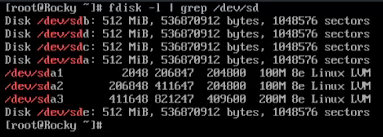
\includegraphics{1.png}
	\item Создайте на каждом из дисков раздел:
	      \\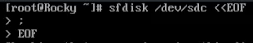
\includegraphics{2.png}
	\item Просмотрите, какие типы партиций, относящиеся к RAID, можно задать:
	      \\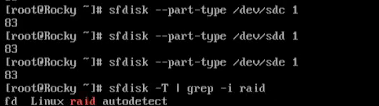
\includegraphics{3.png}
	      \\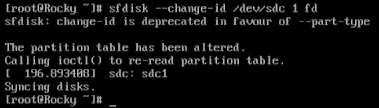
\includegraphics{4.png}
	\item Просмотрите состояние дисков:
	      \\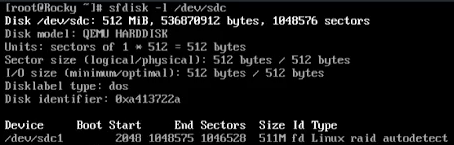
\includegraphics{5.png}
	\item При помощи утилиты \texttt{mdadm} создайте массив RAID 1 из двух дисков:
	      \\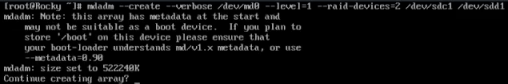
\includegraphics{6.png}
	\item Проверьте состояние массива RAID:
	      \\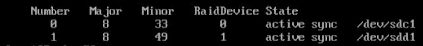
\includegraphics{7.png}
	\item Создайте файловую систему на RAID:
	\item Подмонтируйте RAID:
	      %\\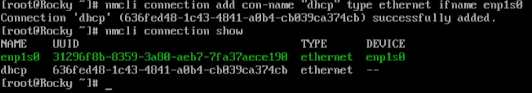
\includegraphics{8.png}
	\item Для автомонтирования добавьте запись в \texttt{/etc/fstab}:
	      %\\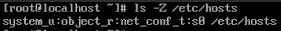
\includegraphics{9.png}
	\item Сымитируйте сбой одного из дисков:
	\item Удалите сбойный диск:
	\item Замените диск в массиве:
	      \\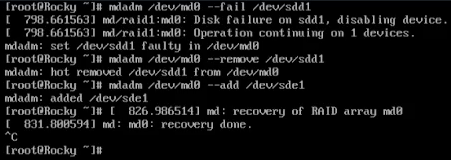
\includegraphics{10.png}
	\item Посмотрите состояние массива:
	      \\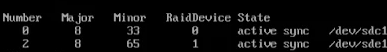
\includegraphics{11.png}
	\item Удалите массив и очистите метаданные:
	      \\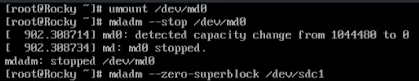
\includegraphics{12.png}
\end{enumerate}

\subsection{RAID-массив с горячим резервом (hotspare)}
\begin{enumerate}
	\item Создайте массив RAID 1 из двух дисков:
	      \\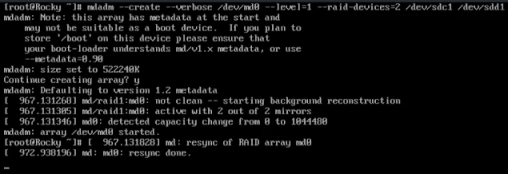
\includegraphics{13.png}
	\item Добавьте третий диск:
	      \\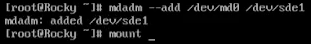
\includegraphics{14.png}
	\item Подмонтируйте \texttt{/dev/md0}:
	\item Проверьте состояние массива:
	      \\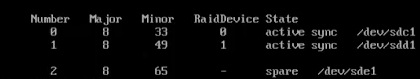
\includegraphics{15.png}
	\item Сымитируйте сбой одного из дисков:
	      \\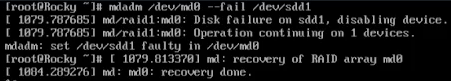
\includegraphics{16.png}
	\item Проверьте состояние массива:
	      \\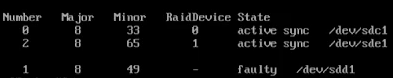
\includegraphics{17.png}
	\item Удалите массив и очистите метаданные:
\end{enumerate}

\subsection{Преобразование массива RAID 1 в RAID 5}
\begin{enumerate}
	\item Создайте массив RAID 1 из двух дисков:
	      \\
\includegraphics{18.png}
	\item Добавьте третий диск:
	      \\
\includegraphics{19.png}
	\item Подмонтируйте \texttt{/dev/md0}:
	\item Проверьте состояние массива:
	      \\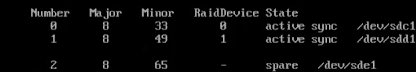
\includegraphics{20.png}
	\item Измените тип массива RAID:
	      \\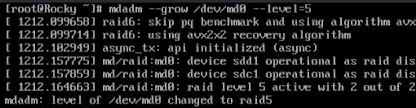
\includegraphics{21.png}
	\item Проверьте состояние массива:
	      \\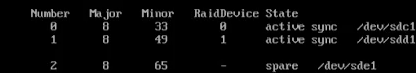
\includegraphics{22.png}
	\item Измените количество дисков в массиве RAID 5:
	      \\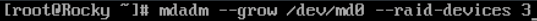
\includegraphics{23.png}
	\item Проверьте состояние массива:
	      \\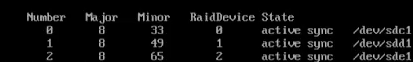
\includegraphics{24.png}
	\item Удалите массив и очистите метаданные:
	\item Закомментируйте запись в \texttt{/etc/fstab}:
\end{enumerate}

\section{Контрольные вопросы}
\begin{enumerate}
	\item Приведите определение RAID. \\
	      RAID (англ. Redundant Array of Independent Disks — избыточный массив независимых (самостоятельных) дисков) — технология виртуализации данных для объединения нескольких физических дисковых устройств в логический модуль для повышения отказоустойчивости и (или) производительности.
	\item Какие типы RAID-массивов существуют на сегодняшний день? \\
	      Де факто стандарт:
	      \begin{itemize}
		      \item RAID 1 — зеркальный дисковый массив;
		      \item RAID 2 — зарезервирован для массивов, которые применяют код Хемминга;
		      \item RAID 3 — дисковый массив с выделенным диском чётности;
		      \item RAID 4 — дисковый массив с чередованием и выделенным диском чётности;
		      \item RAID 5 — дисковый массив с чередованием, в том числе данных чётности (нет диска, выделенного для хранения чётности — блоки чётности чередуются с блоками данных на каждом диске).

	      \end{itemize}
	      Среди современных реализаций массивов RAID представлены дополнительные уровни спецификации:
	      \begin{itemize}
		      \item RAID 0 — дисковый массив повышенной производительности с чередованием без отказоустойчивости;
		      \item RAID 6 — дисковый массив с чередованием, использующий две контрольные суммы, вычисляемые двумя независимыми способами;
		      \item RAID 10 — массив RAID 0, построенный из массивов RAID 1;
		      \item RAID 50 — массив RAID 0, построенный из массивов RAID 5;
		      \item RAID 60 — массив RAID 0, построенный из массивов RAID 6;
		      \item RAID 1E — зеркальный массив из трёх других массивов: RAID 50, RAID 05, RAID 60 и другие.
	      \end{itemize}
	\item Охарактеризуйте RAID 0, RAID 1, RAID 5, RAID 6, опишите алгоритм работы,
	      назначение, приведите примеры применения \\
	      \begin{itemize}
		      \item RAID 0 (striping — <<чередование>>)
		            --- дисковый массив из двух или более жёстких дисков без резервирования.
		            Информация разбивается на блоки данных фиксированной длины и записывается
		            на оба/несколько дисков поочередно.
		      \item RAID 1 (mirroring --- <<зеркалирование>>)
		            --- массив из двух (или более) дисков, являющихся полными копиями друг друга.
		      \item RAID 5
		            --- дисковый массив с чередованием блоков данных и контролем чётности.
		            Блоки данных и контрольные суммы циклически записываются на все диски массива,
		            нет асимметричности конфигурации дисков.
		            Под контрольными суммами подразумевается результат операции XOR (исключающее или).
		      \item RAID 6
		            --- массив из четырёх или более дисков с проверкой чётности P+Q или DP,
		            разработанный для защиты от потери данных при выходе из строя
		            сразу двух жестких дисков в массиве.
		            Варианты RAID 6:
		            \begin{itemize}
			            \item P+Q
			                  --- массив с двумя томами чётности <<P>> и <<Q>>,
			                  по архитектуре RAID 6 P+Q представляет собой расширение RAID 5
			                  с дополнительным диском <<Q>>;
			            \item DP (англ. Dual Parity, Double Parity) — массив с двойной чётностью.
		            \end{itemize}
	      \end{itemize}
\end{enumerate}

\section{Вывод}
В ходе выполнения данной работы я освоил работу с RAID-массивами при помощи утилиты \texttt{mdadm}.

\end{document}
